\section{问题三 储能协同优化}

\subsection{建模与求解}

问题三承接前两问的调度结论，以前问输出的逐时设施负荷（$Total\_Load=IT\times PUE$）为给定输入，在此基础上引入储能，设计充放电策略与购售电、新能源分配方案，同时分析储能对运行成本、碳排放、峰值净购电功率与负荷波动四项指标的影响，本问不再涉及任务调度。与问题一、二含0-1整数变量的调度MILP不同，本问全部决策量为连续非负变量、全部约束为线性等式或不等式、目标函数是购售电净成本的线性函数，故该问题本质上是连续线性规划（LP）问题，无需引入整数变量，也不依赖启发式搜索。其核心难点有二：一是储能充放电、购售电与新能源消纳三类决策需同时满足功率平衡约束与SOC递推关系，彼此紧密耦合；二是碳排放约束与成本最小化之间存在内在张力——降本倾向引导峰谷套利，碳排放却受刚性约束限制，二者在受限消纳下可能冲突。

我们先对储能影响机制做定性分析。低价充电、高价放电的峰谷套利能够降低成本，理论上还兼具削峰与促进新能源消纳的潜力，但在碳排放约束与受限消纳下，这些潜力均受到抑制，并且碳排放约束可能迫使储能改在低碳时段充电，压缩降本空间。另外，受线路容量等物理限制，储能无法无限替代购电，导致碳排放的压降空间也相应有限。面对储能放电可替代购电的情况，碳约束往往使得购电集中在碳强度最高的时段，而这些高碳时段又正是负荷高峰，削峰空间因此受限。不仅如此，峰谷套利天然遵循低买高卖，很可能放大而非平抑净购电的峰谷差异。基于此，我们随后建立LP模型对上述判断做定量验证。

\medskip\noindent\textbf{决策变量。}决策变量为购电量$G_t$、售电量$S_t$、新能源直供量$R_t$、电网充电量$C^g_t$、新能源充电量$C^r_t$、放电量$D_t$（单位MW）与时段末电量$E_t$（MWh），时段$t=0,1,\ldots,2405$；$E_{-1}=Initial$为初始电量。这些变量均连续非负，每区域共$7\times2406$个，构成解空间。

\medskip\noindent\textbf{目标函数。}本模型的优化目标为运行成本最小化，即全时段购电支出扣除售电收入后的净成本最小，其中结清段为 $t=2400\sim2405$。

\begin{equation}
\min \; Z = \sum_{t=0}^{2405} \bigl(G_t \cdot Price_t - S_t \cdot SellPrice_t\bigr)
\end{equation}

其中 $Price_t$ 为逐时购电电价，单位元/MWh，$SellPrice_t$ 为逐时售电电价。储能充放电效率乘积为$\eta_c\eta_d\approx0.86<1$，同时充放属于纯能量损耗。在成本最小化目标下，这一行为会被 LP 自动排除，无需显式约束。

\medskip\noindent\textbf{约束条件。}本模型共包含七类约束条件，依次为功率平衡、受限消纳、SOC递推、SOC边界与终态、充放功率、购售电边界与碳排放限额，分别说明如下。

\textbf{C1\quad 功率平衡约束。}在每个时段，各区域负荷必须由电网购电、新能源直供或储能放电满足。多余功率则可用于储能充电或上网售电。
\begin{equation}
G_t + R_t + D_t = Load_t + C^g_t + C^r_t + S_t \quad \forall t
\end{equation}

\textbf{C2\quad 受限消纳约束。}新能源的直供与充电量之和不得超过该区域逐时消纳能力上限。
\begin{equation}
R_t + C^r_t \le Cap^{renew}_t \quad \forall t
\end{equation}
消纳上限$Cap^{renew}_t$取基准轨迹中该时段实际消纳的新能源量（直供量加基准储能充电量），代表该区域的消纳能力假设。我们以基准观测值作保守估计，避免在缺少拓扑数据时无根据地放大消纳能力。敏感性对照中，放开至可用量$R_t+C^r_t\le Avail_t$时，因可用新能源均值恒大于负荷峰值，购电趋近于零、成本趋近理想下界，该结果脱离工程现实，故正文以受限消纳为主、自由消纳仅作对照。

\textbf{C3\quad 储能SOC递推约束。}时段 $t$ 末的储能电量等于充电量与放电量的差值加上上一时段末的电量，其中充电量经充电效率缩小，放电量经放电效率放大。
\begin{equation}
E_t = E_{t-1} + \eta_c\,(C^g_t + C^r_t) - \frac{D_t}{\eta_d} \quad \forall t
\end{equation}
该递推将各时段储能状态在时间维度上串联，从而使当前充电决策提升后续时段放电能力，反之亦然。

\textbf{C4\quad SOC边界与终态约束。}储能电量须在允许范围内，且末段 $t=2405$ 的电量不低于初始值，防止方案透支储能电量获取短期收益，保证方案可重复执行。
\begin{equation}
E_{\min} \le E_t \le Cap \quad \forall t; \qquad E_{2405} \ge Initial
\end{equation}

\textbf{C5\quad 充放功率约束。}充电总功率和放电功率须在储能设备额定功率范围内。
\begin{equation}
C^g_t + C^r_t \le P^{ch},\quad D_t \le P^{dis} \quad \forall t
\end{equation}

\textbf{C6\quad 购售电边界约束。}购售电量受电网互联容量和售电协议限制。
\begin{equation}
G_t \le MaxGridImport_r,\quad S_t \le SellLimit_r \quad \forall t
\end{equation}

\textbf{C7\quad 碳排放$\varepsilon$约束，主时域。}我们定义购电碳排放总量不超过碳基准排放量$\varepsilon$倍的约束为碳排放$\varepsilon$约束，后文简称$\varepsilon$约束，作用于主时域$t=0,\ldots,2399$。
\begin{equation}
\sum_{t=0}^{2399} G_t \cdot CI_t \le 10^3 \cdot \varepsilon \cdot CarbonBase_r
\end{equation}
其中$CI_t$为逐时碳强度（tCO$_2$/MWh），$CarbonBase_r$为区域$r$的碳基准排放量（kt），$10^3$为kt到tCO$_2$换算因子。$\varepsilon=1.00$档的解可行且唯一，后文称此解为主解；逐档检验表明$\varepsilon<1.00$在六区域全部无可行解，碳排放已逼近可行域下限。

综上所述，我们建立储能协同优化线性规划模型如下。

\begin{equation}
\begin{aligned}
\min \quad & Z = \sum_{t=0}^{2405} \bigl(G_t \cdot Price_t - S_t \cdot SellPrice_t\bigr) \\
\text{s.t.} \quad & G_t + R_t + D_t = Load_t + C^g_t + C^r_t + S_t \quad \forall t \\
& R_t + C^r_t \le Cap^{renew}_t \quad \forall t \\
& E_t = E_{t-1} + \eta_c\,(C^g_t + C^r_t) - D_t/\eta_d \quad \forall t \\
& E_{\min} \le E_t \le Cap \quad \forall t;\quad E_{2405} \ge Initial \\
& C^g_t + C^r_t \le P^{ch},\quad D_t \le P^{dis} \quad \forall t \\
& G_t \le MaxGridImport_r,\quad S_t \le SellLimit_r \quad \forall t \\
& \sum_{t=0}^{2399} G_t \cdot CI_t \le 10^3 \cdot \varepsilon \cdot CarbonBase_r,\quad \varepsilon=1.00 \\
& G_t, S_t, R_t, C^g_t, C^r_t, D_t, E_t \ge 0 \quad \forall t
\end{aligned}
\end{equation}

\medskip\noindent\textbf{求解策略。}该模型为连续LP，每区域约有$7\times2406$个连续变量，约束均为线性。我们用开源求解器HiGHS（scipy.optimize.linprog）对六区域独立求解，$\varepsilon=1.00$下均求得最优可行解。模型一致性三项检验全部通过，包括同时刻充放电均为零、SOC终态合规，以及功率平衡残差约$1\times10^{-13}$\,MW（数值误差量级）。

\subsection{结果与影响分析}

\medskip\noindent\textbf{主解结果。}我们用 HiGHS 求解器计算上述模型，得到各区域最优解。在满足碳排放约束 $\varepsilon=1.00$ 的条件下，六区域聚合运行成本为\textbf{2213.35 M元}，总碳排放为\textbf{2044.79 kt}，分区域结果见表 \ref{tab:s3-main}。

\begin{table}[ht]
\centering
\footnotesize
\caption{储能协同优化主解结果（受限消纳，$\varepsilon=1.00$，主时域0--2399 h）}
\label{tab:s3-main}
\begin{tabular}{lcccccc}
\toprule
区域 & 成本（M元） & 碳排放（kt） & 峰值净购电（MW） & 净购电std（MW） & SOC利用率 & 储能充放贡献 \\
\midrule
A & 617.94 & 581.27 & 550.0 & 115.34 & 8.47\% & -- \\
B & 567.59 & 519.70 & 520.0 & 105.46 & 9.97\% & -- \\
C & 542.15 & 483.82 & 510.0 & 101.05 & 11.79\% & -- \\
D & 225.46 & 262.39 & 510.0 & 153.15 & 24.76\% & -- \\
E & 114.73 & 84.56 & 370.0 & 121.67 & 35.98\% & -- \\
F & 145.48 & 113.06 & 340.0 & 117.37 & 34.02\% & -- \\
\midrule
\textbf{聚合} & \textbf{2213.35} & \textbf{2044.79} & \textbf{550.0} & 686.15 & 20.83\% & 99.36 \\
\bottomrule
\end{tabular}
\end{table}

D/E/F区储能利用率24.8\%--36.0\%，显著高于A/B/C区的8.5\%--11.8\%。储能价值高度集中于电价差大、碳强度低的D/E/F区。A/B/C区储能近乎闲置，SOC长期维持在初始值附近。在$\varepsilon$约束与受限消纳的双重限制下，套利空间被大幅压缩。图 \ref{fig:s3-soc} 给出六区域SOC与充放功率的全时序轨迹，直观印证了这一区域差异。

\begin{figure}[ht]
\centering
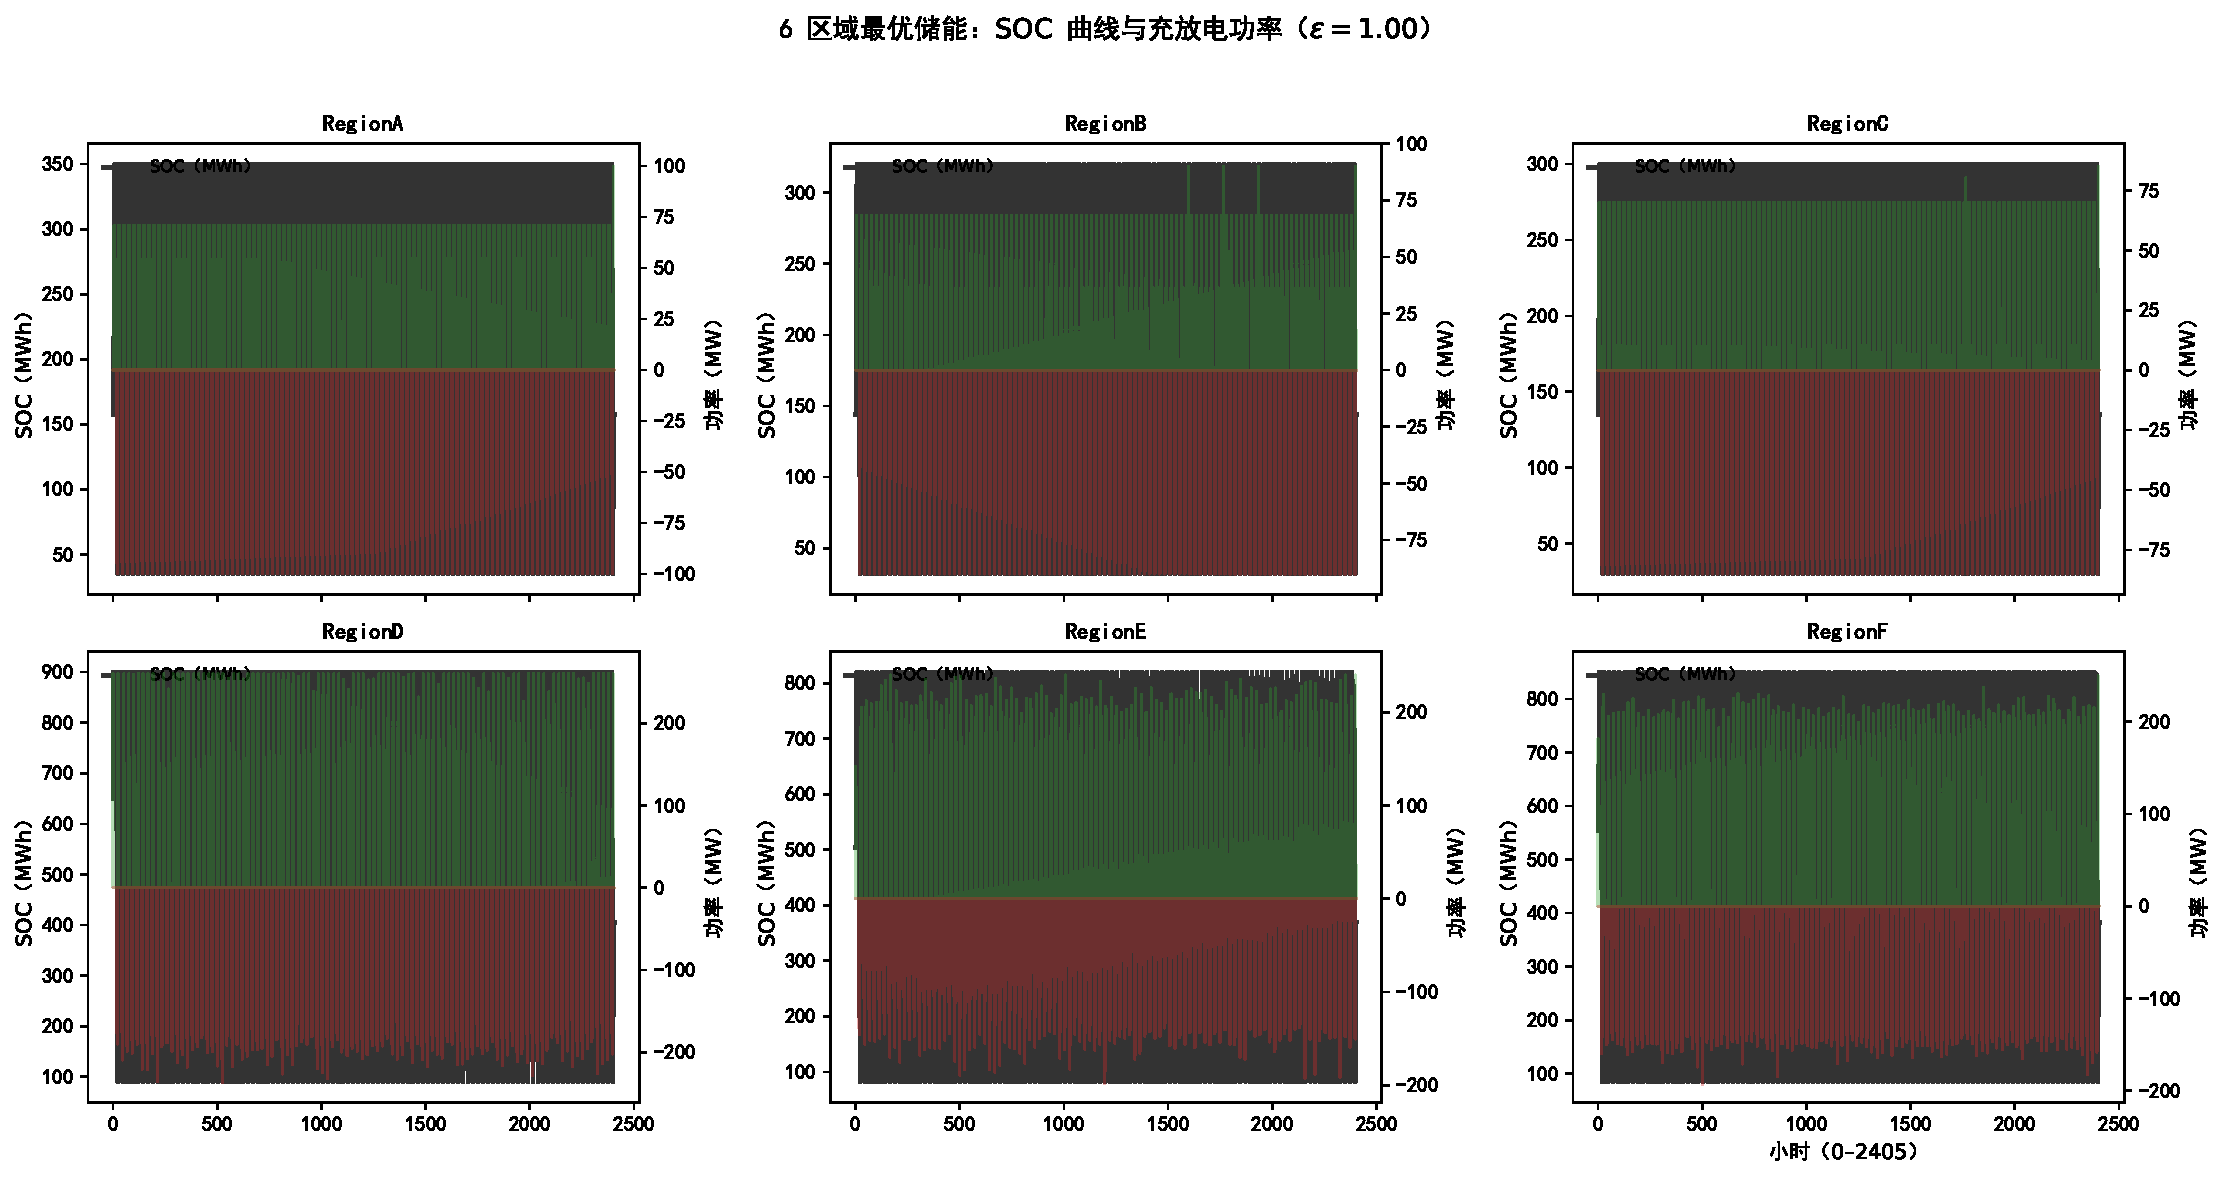
\includegraphics[width=0.95\textwidth]{../../outputs/figures/sub3-soc-charge-discharge-v2.pdf}
\caption{六区域储能SOC与充放功率时序（受限消纳，$\varepsilon=1.00$）（AI 辅助生成）}
\label{fig:s3-soc}
\end{figure}

\medskip\noindent\textbf{储能价值量化与归因拆分。}

为量化储能的真实增益，我们设置无储能对照实验。该对照将充放电变量冻结为$D_t=C^g_t=C^r_t=0$，其余购售电与新能源分配仍可优化（受限消纳、$\varepsilon=1.00$），是无储能条件下的诚实下界。无储能聚合成本2387.86\,M元，储能优化带来的成本节约为

\begin{equation}
\Delta_{total} = 2387.86 - 2213.35 = \mathbf{174.51\;\text{M元}}\;(-7.3\%)
\end{equation}

进一步，我们增设购电时点自由优化但无储能的对照实验，把 174.51 M 元的成本节约拆分为两个独立贡献来源。

\textbf{储能充放电贡献} $\Delta_1 = 99.36$ M 元，占总节约的 56.9\%。这是纯储能充放调度带来的成本下降，即储能通过低价充电、高价放电实现的峰谷套利收益。该行为也称储能时移，指通过充放电把电能从低价或富余时段搬移至高价或紧缺时段使用。

\textbf{购电时点自由化贡献} $\Delta_2 = 75.15$ M 元，占总节约的 43.1\%。即使没有储能设备，仅通过优化购电时点，在低价时段集中购电、高价时段减少购电，即可实现这部分成本下降。该效果本质上是把购电负荷挪到低价时段，与储能把电量从低价时段搬到高价时段的原理一致，但在无储能条件下同样可达。

拆分结果精确吻合，$99.36+75.15=174.51$。其中约57\%来自储能充放电，43\%来自购电时点自由选择，后者不依赖储能物理存在。故评估储能边际经济价值应以充放电贡献99.36\,M元为准。若储能全生命周期成本低于该值，那么引入储能具有合理性，而以174.51\,M元为决策依据会高估真实价值。

\medskip\noindent\textbf{四指标影响逐项分析。}

\textbf{1. 运行成本。显著下降，但降幅受碳排放约束限制。}优化方案较无储能下界降174.51\,M元（$-7.3\%$）。这得益于峰谷套利，即低价充电、高价放电替代购电。但$\varepsilon=1.00$下储能无法在高碳低价时段无限扩充电量，降幅受碳排放刚性限制（下称"碳排放刚性"，指碳排放已逼近物理下限、难以再压缩的性质）；若$\varepsilon>1.00$降本空间更大，碳排放则同步上升。

\textbf{2. 碳排放。几乎无压缩空间，$\varepsilon=1.00$ 即为可行域边界。}优化方案碳排放2044.79\,kt，与碳基准2045.36\,kt几乎持平（仅降0.03\%）。二分法给出各区域$\varepsilon_{\min}$，结果见表 \ref{tab:s3-emin}。A/B/C区0.993--0.994（最多再压降0.6\%--0.7\%），D/E/F区0.957--0.969（可再压降3\%--4\%），且$\varepsilon<1.00$在六区域全部无可行解。这一结果表明，受限消纳下的碳排放已逼近系统结构的物理下限。而基础设施（新能源装机、线路容量）未变，储能只能重新分配已有低碳资源的时点分布，无法凭空产生低碳电力。碳排放刚性是受限消纳与$\varepsilon$约束双重作用的直接后果。

\begin{table}[ht]
\centering
\footnotesize
\caption{各区域碳排放可行域边界$\varepsilon_{\min}$（$\varepsilon$ 约束可收紧极限）}
\label{tab:s3-emin}
\begin{tabular}{lcccccc}
\toprule
区域 & A & B & C & D & E & F \\
\midrule
碳排放下限$C_{\min}$（kt） & 577.47 & 516.49 & 480.95 & 254.88 & 80.96 & 108.72 \\
$\varepsilon_{\min}$ & 0.9935 & 0.9938 & 0.9941 & 0.9693 & 0.9574 & 0.9616 \\
较基准可压降 & $-$0.65\% & $-$0.62\% & $-$0.59\% & $-$3.08\% & $-$4.26\% & $-$3.84\% \\
\bottomrule
\end{tabular}
\end{table}

\textbf{3. 区域峰值净购电功率。削峰存在，但峰值触及购电上限。}优化方案各区域峰值净购电均等于购电上限（A 550、B 520、C 510、D 510、E 370、F 340 MW），触及时段占比8.5\%--17.9\%，集中在碳强度最高的若干小时（如A区Hour 51，电价476.8元/MWh、碳强度0.68 t/MWh）。触及上限是$\varepsilon$约束、受限消纳与负荷刚性三重耦合的必然结果。$\varepsilon$要求总购电碳排放不超过基准，消纳上限锁定了新能源供应，负荷又是给定输入。这样一来，LP无法回避高碳高负荷时段的大功率购电，储能削峰空间被碳约束压缩。这是真实工程代价而非模型缺陷。图 \ref{fig:s3-peak-shaving} 对比了优化方案的峰值净购电与购电上限，可见各区域均顶格触及上限，这表明在碳排放不恶化的前提下，系统无进一步降低峰值净购电的空间。

\begin{figure}[ht]
\centering
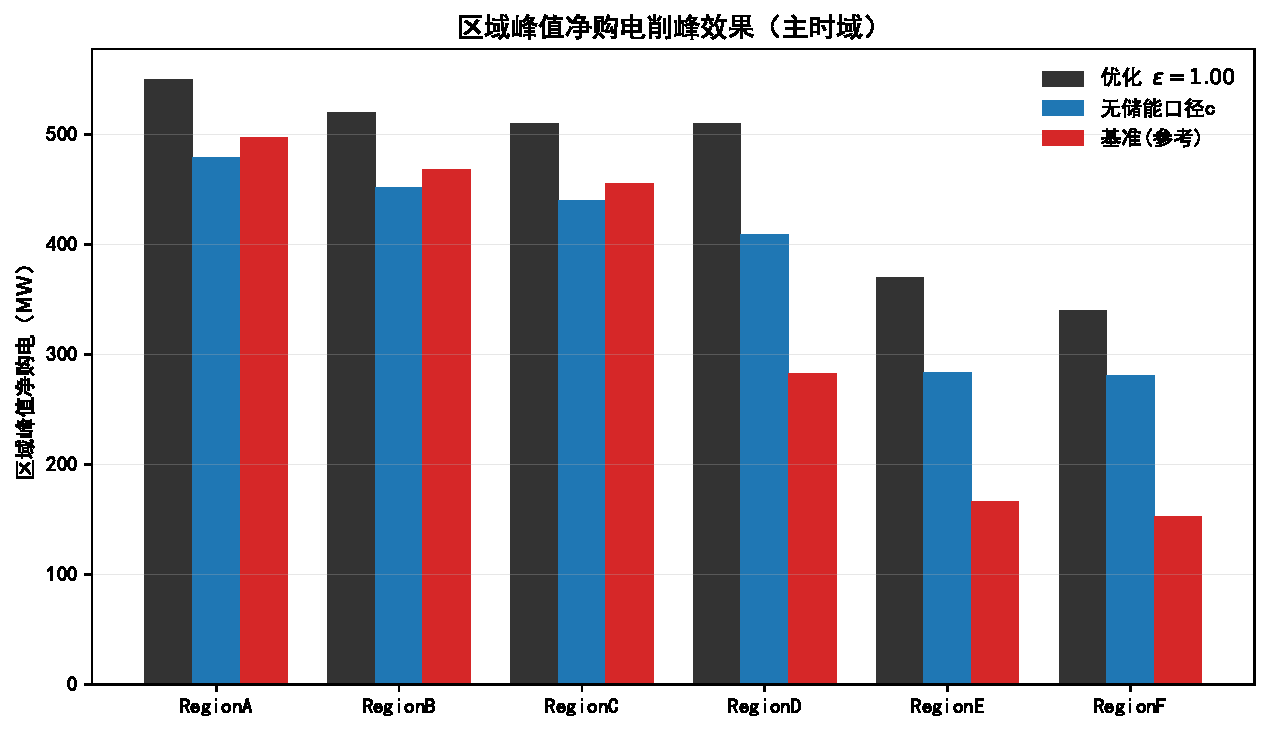
\includegraphics[width=0.85\textwidth]{../../outputs/figures/sub3-peak-shaving-v2.pdf}
\caption{六区域峰值净购电对比（优化方案触及购电上限）（AI 辅助生成）}
\label{fig:s3-peak-shaving}
\end{figure}

\textbf{4. 净购电波动。波动不降反升。}优化方案净购电标准差从365.43升至686.15 MW（+87.7\%），显著恶化。其根源在于成本最小化驱动的峰谷套利：低价时段大量充电拉升购电、高价时段集中放电压低购电，净购电序列的峰谷差因此被放大而非平抑。换言之，单一成本目标下的储能策略天然具有放大器效应，以波动增大换取成本下降；若需平抑波动，须引入多目标优化，如对净购电方差设置惩罚项或直接施加波动约束。需要说明，此处度量对象为净购电序列$G_t-S_t$，而非设施总负荷$Total\_Load$——后者为给定输入、储能无法影响，净购电波动才是储能可作用的电网侧指标。

综合四项指标，受限消纳与碳排放刚性（$\varepsilon=1.00$）下，储能的价值主要体现在降本：通过充放电实现约99.36\,M元成本节约，而碳排放几乎无压缩空间（$\varepsilon_{\min}\approx0.96$--0.99）、峰值净购电触及购电上限、净购电波动在纯成本目标下不降反升。这表明降本、降碳、削峰、平抑波动四个目标存在真实冲突，单一目标模型无法自动兼顾，储能的实际效益取决于运营目标的主次取舍。后续多目标分析将量化刻画这些冲突，并给出折中策略。
